\section{Initial Results}
\label{section_result_initial_results}

This section presents our initial results,
aimed at replicating the findings from \citen{Arthur2023} to ensure the integrity of our implementation.
We tested our algorithm on 100 randomly generated 40x40 perfect mazes \cite{Naeem2021}, incrementing the number of agents from 1 to 40.
We evaluated:

\begin{itemize}
    \item Steps taken by the pioneer (first agent to find the goal).
    \item Fraction explored before the pioneer found the goal.
\end{itemize}

These tests were conducted for three implemented algorithms:

\begin{itemize}
\item Our Algorithm
\item Backward Interval Filling Variation
\item Extended Tarry's Algorithm \cite{Kivelevitch2010}
\end{itemize}

Below, we provide comparative visuals for each algorithm's performance.

Figures \ref{fig_comparison_steps} and \ref{fig_comparison_fraction} show a side-by-side comparison of our results with those from \citen{Arthur2023},
considering the default variation of the algorithm.

\begin{figure}[H]
\centering
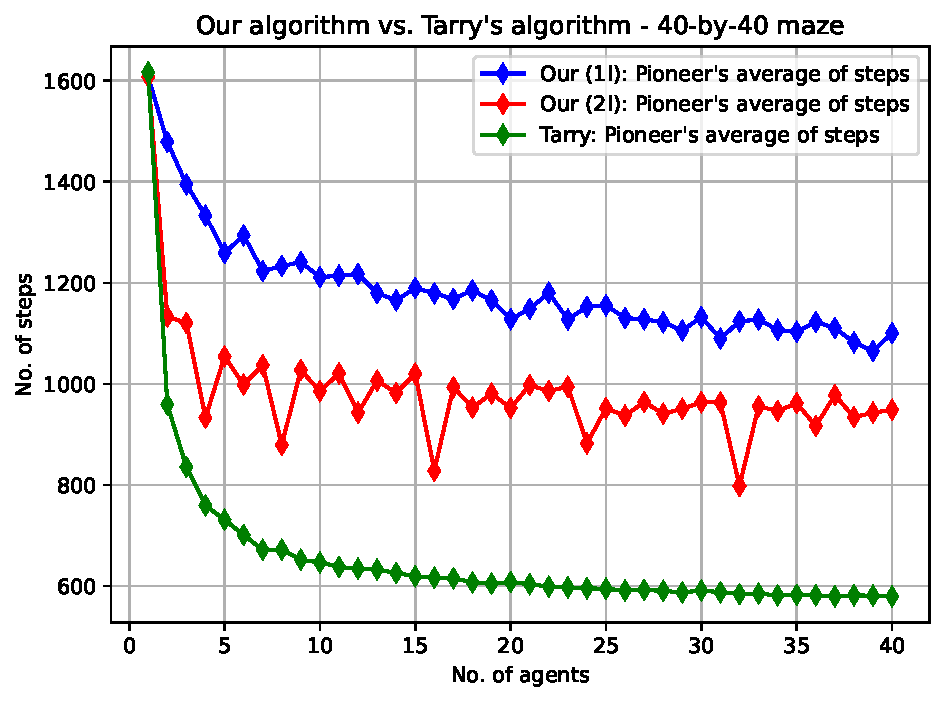
\includegraphics[height=5cm]{Cap3/arthur_tarry_40x40_steps.pdf}
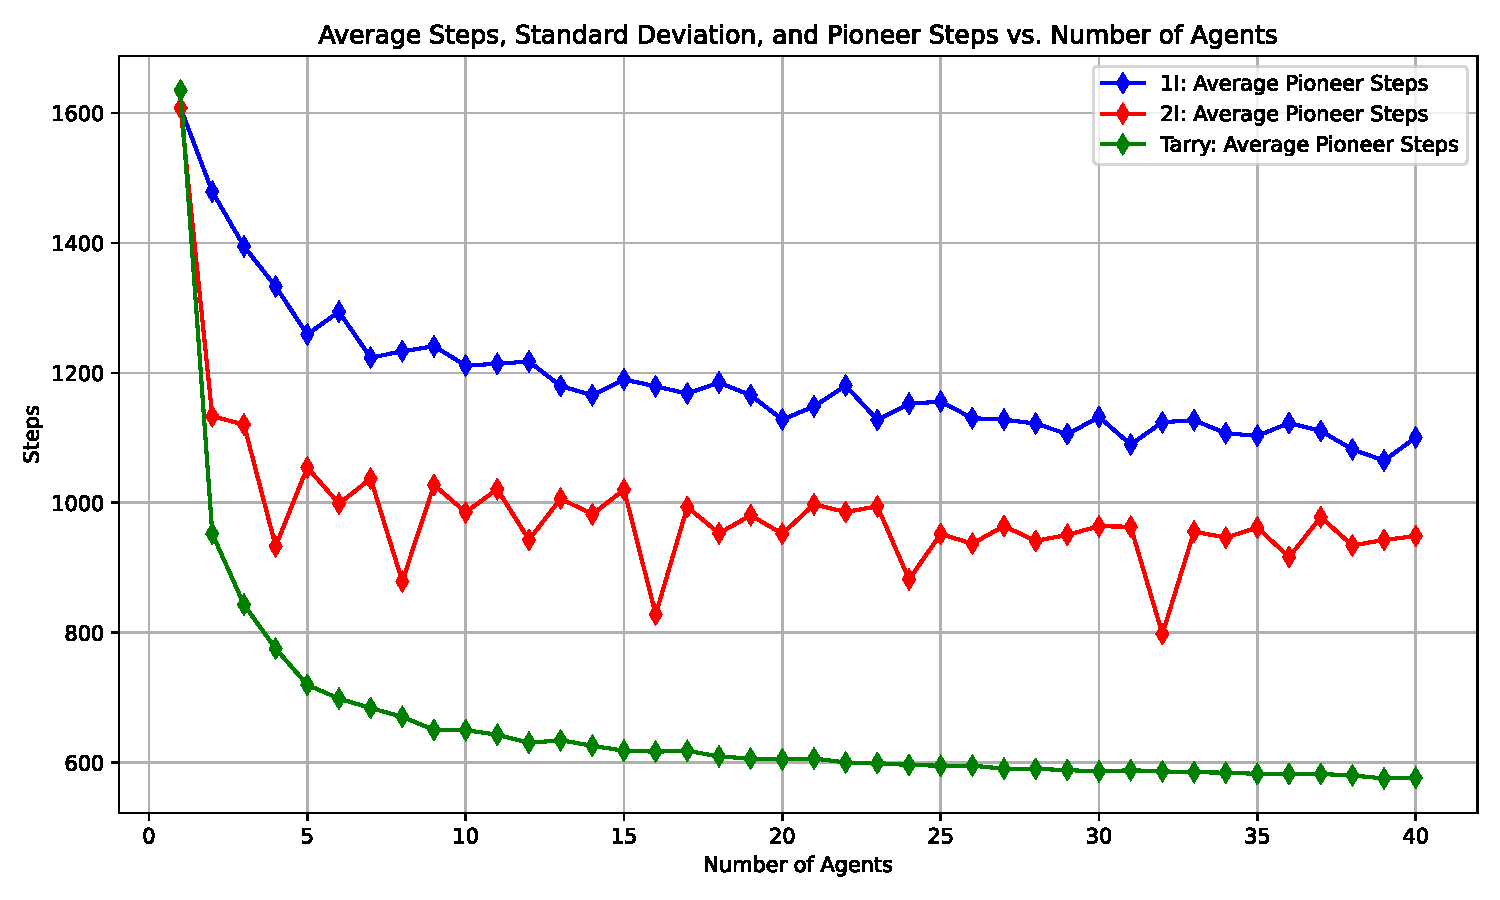
\includegraphics[height=5cm]{Cap3/self_steps_40_by_40_tarry.pdf}
\caption{Comparison of total steps: Left - Results from \citen{Arthur2023}; Right - Our results}
\label{fig_comparison_steps}
\end{figure}

\begin{figure}[H]
    \centering
    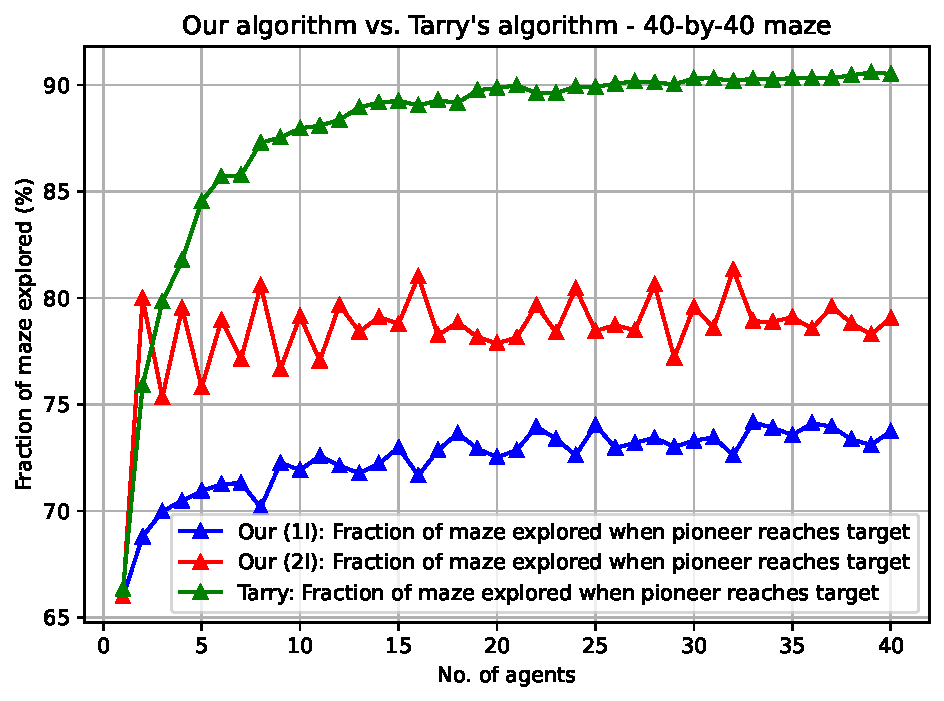
\includegraphics[height=5cm]{Cap3/arthur_tarry_40x40_fraction.pdf}
    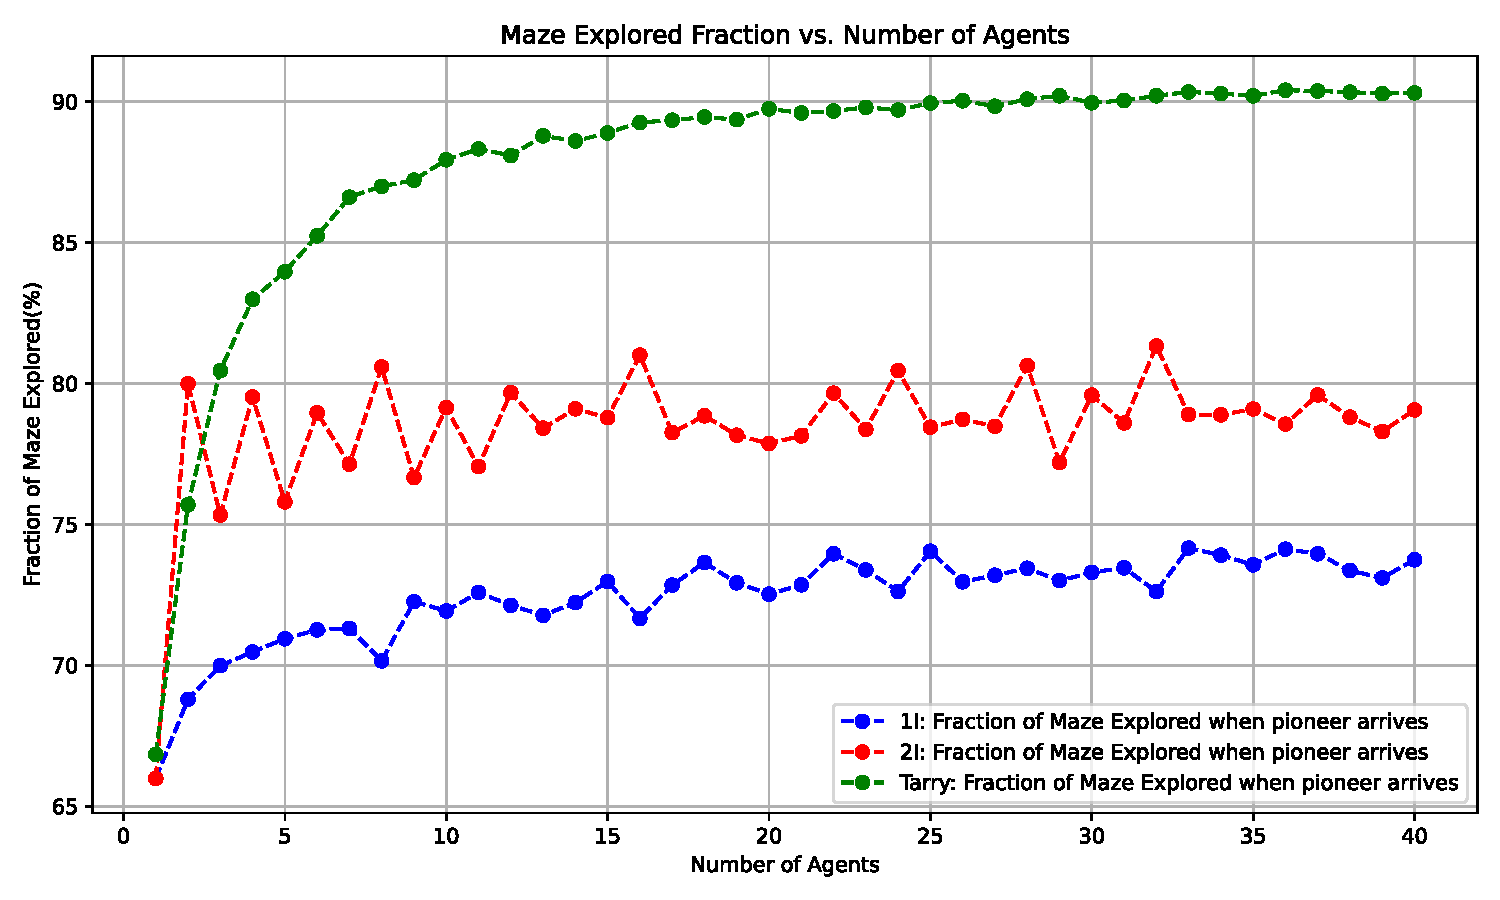
\includegraphics[height=5cm]{Cap3/self_fraction_40_by_40_tarry.pdf}
    \caption{Comparison of explored fraction: Left - Results from \citen{Arthur2023}; Right - Our results}
\label{fig_comparison_fraction}
\end{figure}

As evident from the figures, our results closely match the original findings,
demonstrating that our modifications have not altered the core functionality of the algorithm.

\section{Graph Visualization}
\label{section_result_graph_visualization}

One significant enhancement is the capability to visualize graphs
beyond perfect mazes, expanding our algorithm's applicability to general graphs.

To demonstrate this capability, we applied our algorithm to explore
an imperfect maze, which is a cyclic graph, using three agents. The overall exploration of the maze is depicted in Figure \ref{fig_imperfect_maze_exploration}.

\begin{figure}[H]
\centering
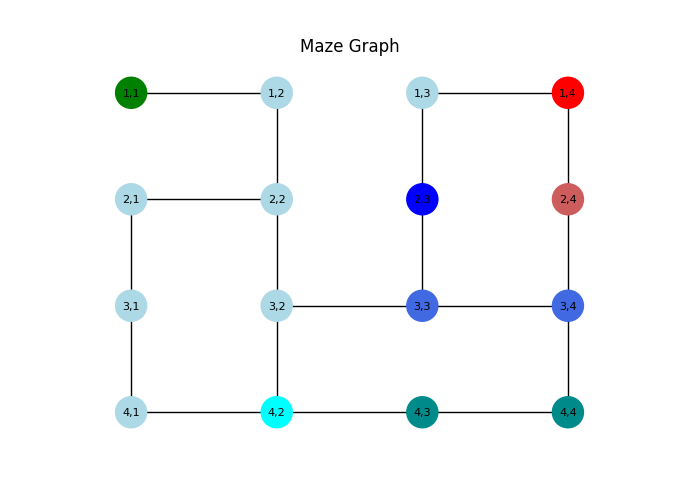
\includegraphics[width=0.5\textwidth]{Cap3/maze_imperfect_exploration.png}
\caption{Exploration of an imperfect maze(graph) by three agents.}
\label{fig_imperfect_maze_exploration}
\end{figure}

This visualization showcases how our algorithm can handle graphs
with cycles, illustrating the adaptability of our approach.
To enable comparisons with our previous work on perfect mazes,
we developed utilities to convert between the old and new graph formats.

\section{Agent Tree Visualization}
\label{section_result_tree_visualization}

In addition to overall graph exploration,
we enhanced our implementation to visualize the individual trees constructed by each agent during the exploration process.
These trees reflect the paths taken by agents, incorporating features such as handling
cycles and displaying intervals for each node.

The Figures \ref{fig_agent_1_tree}, \ref{fig_agent_2_tree} and \ref{fig_agent_3_tree}
show the trees constrcuted by the 3 agents for the exploration displayed in Figure \ref{fig_imperfect_maze_exploration}.
    
\begin{figure}[H]
\centering
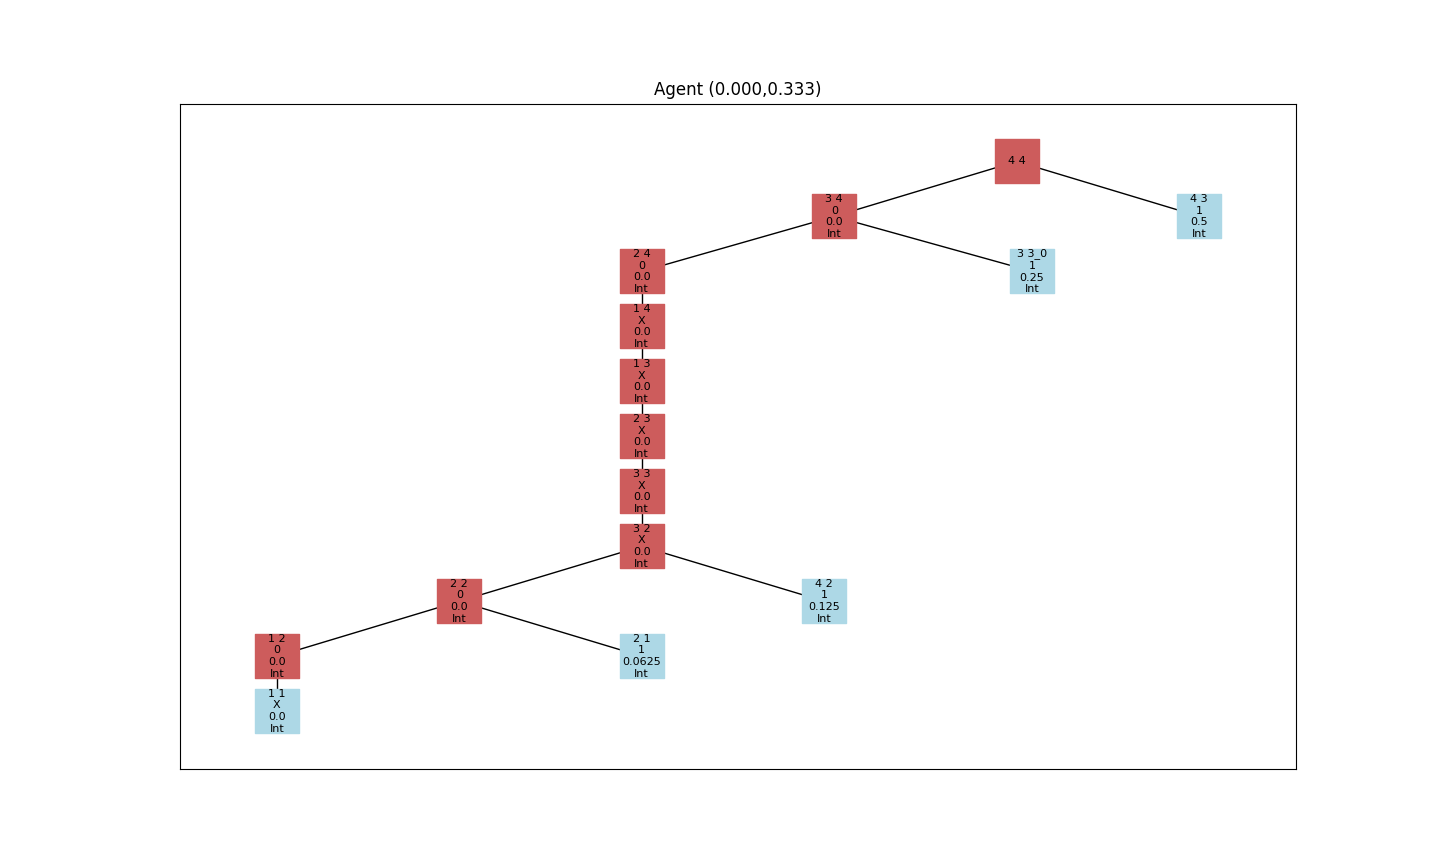
\includegraphics[width=1\textwidth]{Cap3/agent_1.png}
\caption{Trees constructed by agent post-exploration: \textbf{Agent 1}.}
\label{fig_agent_1_tree}
\end{figure}

\begin{figure}[H]
\centering
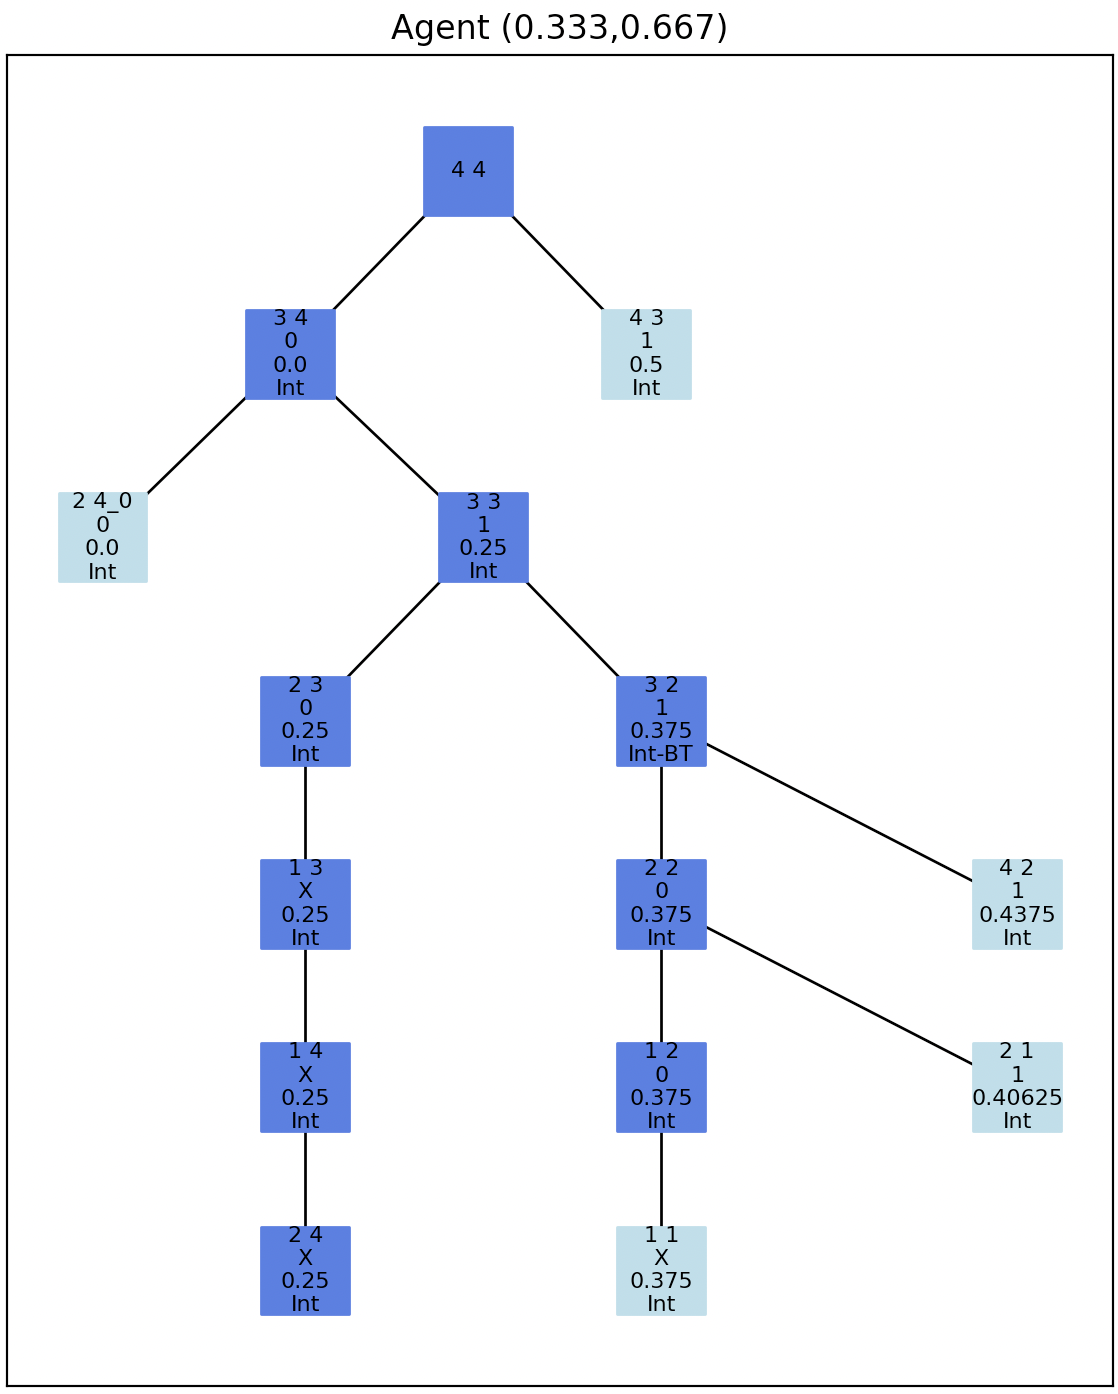
\includegraphics[width=1\textwidth]{Cap3/agent_2.png}
\caption{Trees constructed by agent post-exploration: \textbf{Agent 2}.}
\label{fig_agent_2_tree}
\end{figure}

\begin{figure}[H]
\centering
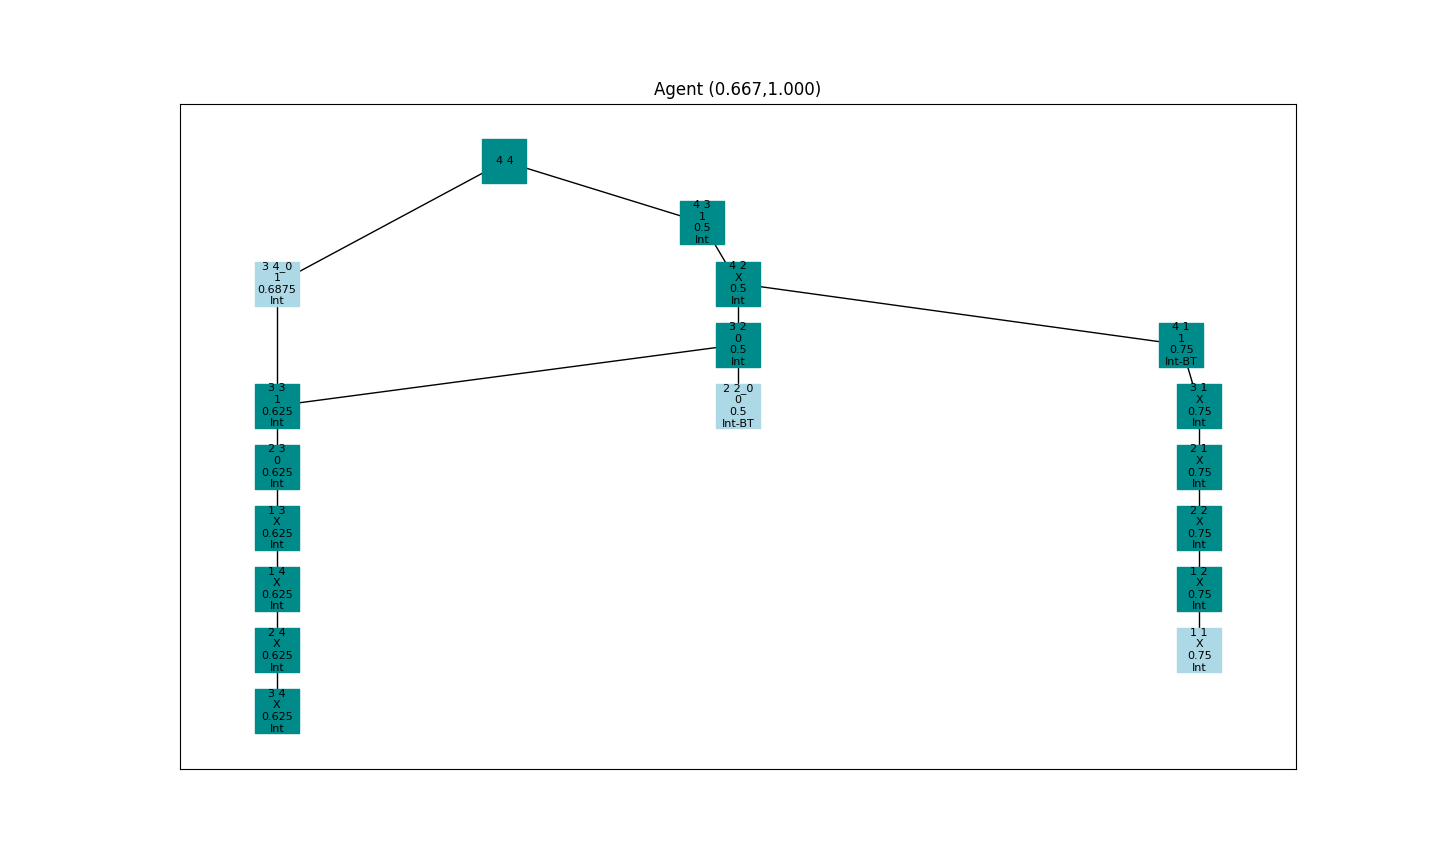
\includegraphics[width=1\textwidth]{Cap3/agent_3.png}
\caption{Trees constructed by agent post-exploration: \textbf{Agent 3}.}
\label{fig_agent_3_tree}
\end{figure}
    
These visualizations illustrate how each agent independently constructs its own representation of the graph,
adapting to the imperfections and resulting in different exploration paths.
    
    
    
    
    
    